\NeedsTeXFormat{LaTeX2e}
\documentclass	[12pt]{article}
\usepackage[pdftex]{color,graphicx}

\usepackage{graphicx,caption,subcaption}
\begin{document}

\title{\bf{Integrated Data Analysis of the DIII-D Density Profile}}
\author{L. Stagner \& W.W. Heidbrink \\ University of California--Irvine, Irvine, California, USA}
\date{}
\maketitle
\begin{abstract}
\end{abstract}
\section{Introduction}
Introstuff

\section{Integrated Data Analysis}
As fusion experiments expand, so does the number of diagnostics used to probe the underlying physics. With the increase in diagnostics the number of interrelations among the diagnostics increases accordingly. While each diagnostic can act independently it is often advantageous to combine the data sets to acquire the most accurate result that is consistent with all the information available. This causes difficulties when trying to combine multiple data sets that cover complementary areas of interest. Bayesian data analysis give a comprehensive, scalable, and automated framework for combining complementary diagnostics.    
\subsection{The Bayesian perspective}
Bayesian statistics differs from the prevailing frequentist statistics that is taught in most introductory courses. The difference between the two views is in the definition of probability. In the Bayesian perspective, probability represented a degree of belief or plausibility that an event was true, based on the information available. This school of thought is opposed to frequentist view that probability is a long run relative frequency with which the event occurs, given infinitely many repeated experimental trials.\cite{von2011bayesian}

While the frequentist view is seemingly more objective, it is limited in its straightforward application since some things cannot have long run relative frequencies and, as a result, cannot be analysed by probability theory. For instance a constant, such as the mass of an object, cannot be analysed by a straightforward application of the frequentist definition of probability as a long run relative frequency. To use the frequentist view you first have to relate the mass to the data through some function called the \emph{statistic}. Since statistic is subject to random noise it becomes the random variable to which the rules of probability can then be applied. The issue with this approach is that there is no natural way of choosing the best statistic. The founders of the field have a plethora of ad hoc rules and tests to determine which statistic should be used in any situation. These rules and tests hides much of the mechanics and assumptions inherent in the analysis and the consequences can often turn up at the worst possible moments.\cite{sivia2006data}

The bayesian definition has no such difficulty since nearly anything can be thought of as a probability and the framework formulates all assumptions to be explicit. That is not to say that it is without its issues. The frequentist view is often much easier to use because it hides most of the difficulties from the user. In bayesian statistics you have to be very careful with the assumptions that are made since it can drastically affect the results. Also, the calculation of optimal parameters is also a challenging numerical exercise in Bayesian statistics. It was partially for this reason that the frequentist view arose into prominence. It was only in the mid 20th century with the advent of computers and efficient sampling algorithms that Bayesian statistics has begun its resurgence. In recent years Bayesian analysis has become essential to many scientific fields such as cosmology and artificial intelligence.\cite{von2011bayesian}
\subsection{Mathematical Formulation}
stuff
\subsection{Principle of Maximum Entropy}
stuff
\subsection{Combining multiple diagnostics}
stuff
\subsection{Model Comparison}

\section{Forward modelling of density diagnostics}
stuff
\subsection{Functional form of the density profile}
stuff
\subsection{Interferometry}
stuff
\subsection{Reflectometry}
stuff
\subsection{Thomson scattering}
stuff
\subsection{Beam emission spectroscopy}
stuff
\section{Likelihood and prior probabilities}
stuff
\subsection{Priors}
stuff
\subsubsection{Parameter space priors}
stuff
\subsubsection{Data space priors}
stuff
\subsection{Likelihoods}
stuff
\subsubsection{Interferometry}
stuff
\subsubsection{Reflectometry}
stuff
\subsubsection{Thomson scattering}
stuff
\subsubsection{Beam emission spectroscopy}
stuff
\subsubsection{Combined likelihood probability}
stuff
\section{Total posterior probability}
stuff
\subsection{Exploring the posterior}
stuff
\section{Representation of Error}
stuff
\section{Density profile reconstructions}
stuff
\subsection{H-mode reconstruction}
stuff
\begin{figure}[ht]
	\centering
	\includegraphics[width=12cm,keepaspectratio=true]{figures/bfit146102_00505_all5}
	\vspace{-30pt}
	\caption{Reconstruction}
\label{hi}
\end{figure}
otherstuff
\subsection{L-mode reconstruction}
stuff
\section{Determining discrepant diagnostics}
stuff
\begin{figure}[h!]
	\centering
	\begin{subfigure}[b]{0.5\textwidth}
		\centering
		\includegraphics[width=\textwidth,keepaspectratio=true]{figures/bfit146102_00505_thom5}
		\vspace{-30pt}
		\caption{Thomson scattering}
		\label{fig:ts505}
	\end{subfigure}
	\hspace{-20pt}
	\begin{subfigure}[b]{0.5\textwidth}
		\centering
		\includegraphics[width=\textwidth,keepaspectratio=true]{figures/bfit146102_00505_inter5}
		\vspace{-30pt}
		\caption{Interferometer}
		\label{fig:inter505}
	\end{subfigure} \\%  ------- End of the first row ----------------------%
	\begin{subfigure}[b]{0.5\textwidth}
		\centering
		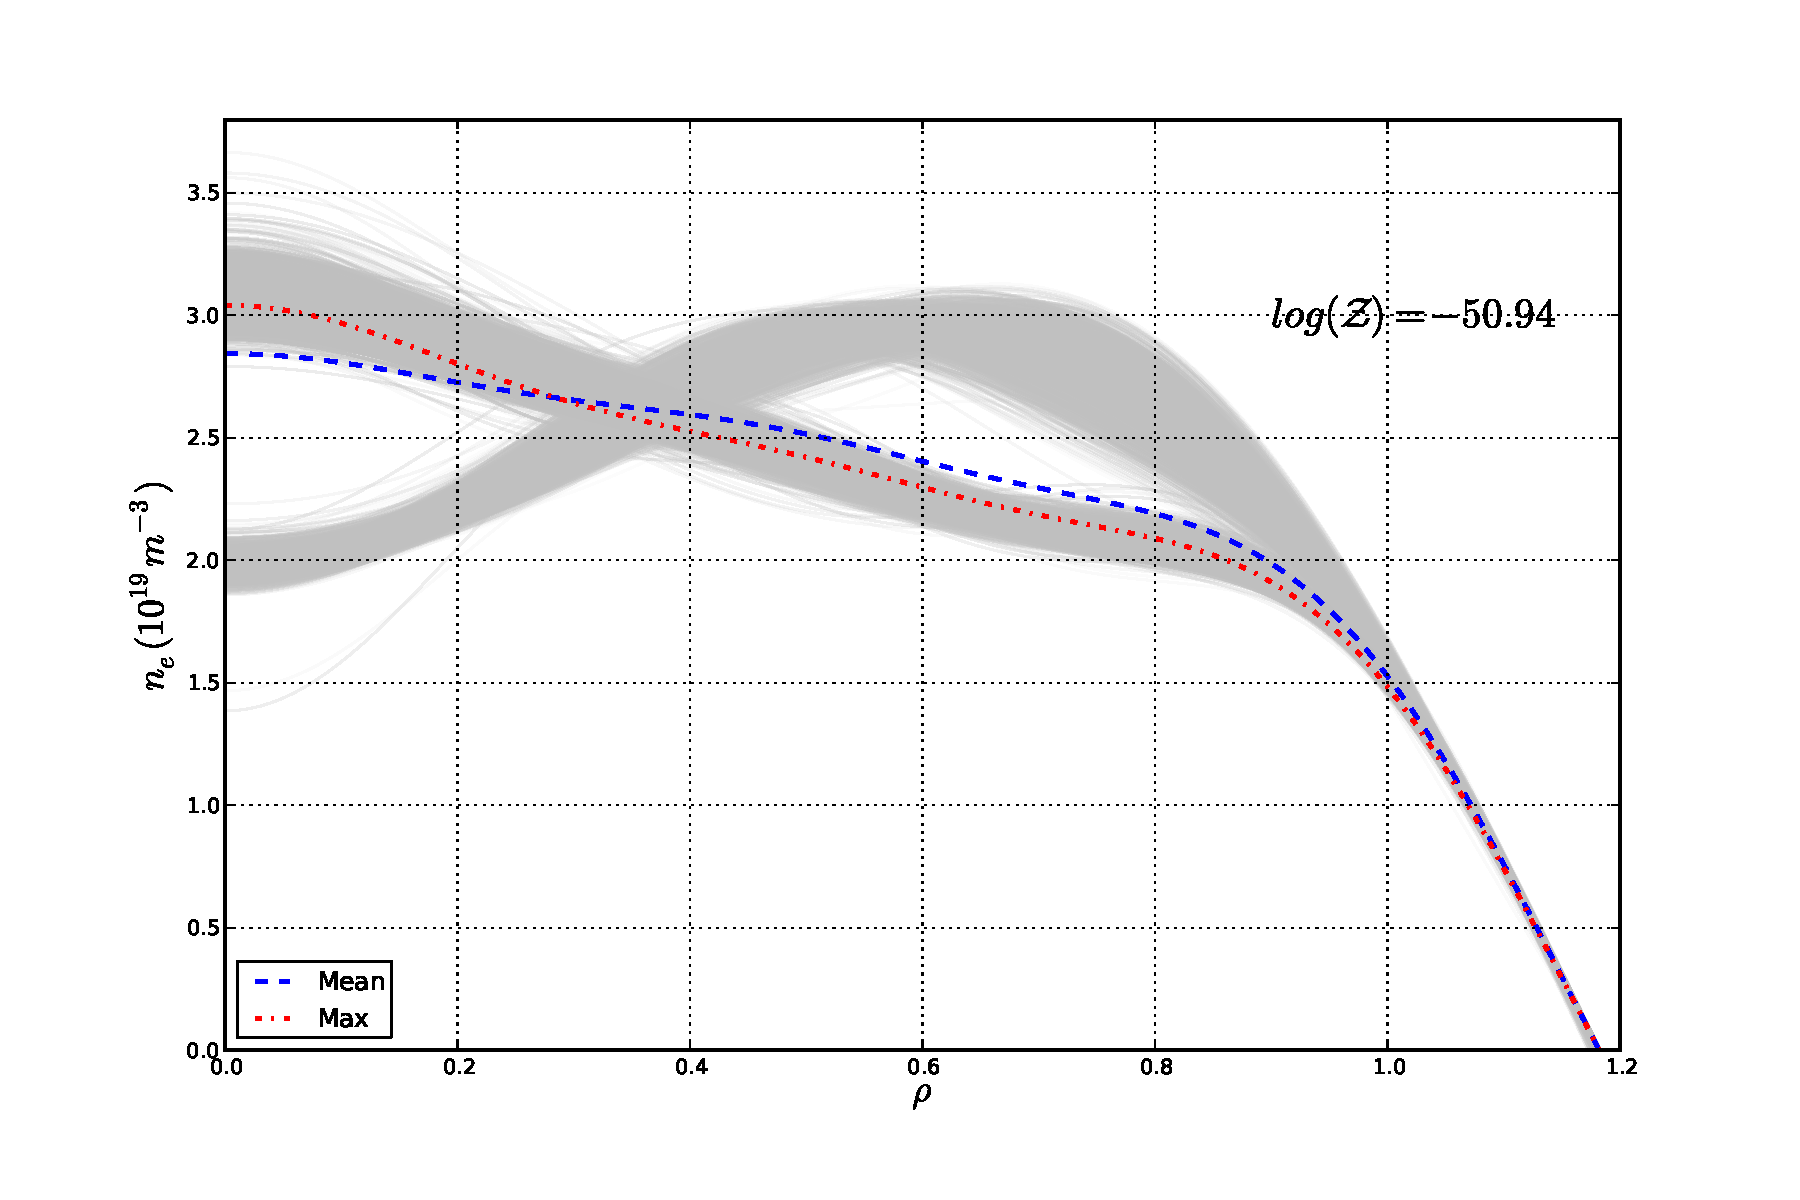
\includegraphics[width=\textwidth,keepaspectratio=true]{figures/bfit146102_00505_refl5}
		\vspace{-30pt}
		\caption{Reflectometry}
		\label{fig:refl505}
	\end{subfigure}
	\hspace{-20pt}
	\begin{subfigure}[b]{0.5\textwidth}
		\centering
		\includegraphics[width=\textwidth,keepaspectratio=true]{figures/bfit146102_00505_all5}
		\vspace{-30pt}
		\caption{Combined}
		\label{fig:all505}
	\end{subfigure}
	\caption{The l-o-n-g caption for all the subfigures (FirstFigure through FourthFigure) goes here.}
	\label{fig:dne505}
\end{figure}
\section{Conclusions and future work}
stuff

\bibliographystyle{unsrt}
\bibliography{bayes,algorithms,diag}
\end{document}
